%%%%%%%%%%%%%%%%%%%%%%%%%%%%%%%%%%%%%%%%%%%%%%%%%%%%%%%%%%%%%%%%%%%%%%%%%%%%%%%
%% PROJECT OVERVIEW:
%%%%%%%%%%%%%%%%%%%%%%%%%%%%%%%%%%%%%%%%%%%%%%%%%%%%%%%%%%%%%%%%%%%%%%%%%%%%%%%
% The goal of this project is for you to further explore a certain subject that we covered
% in class or a new subject related to it (based on some previous work). This is an open
% project in a sense that you will propose the problem you would like to work on and the
% solution you are planning use. Your main goal should be to explore the characteristics of
% your problem/solution under the reinforcement learning framework
%%%%%%%%%%%%%%%%%%%%%%%%%%%%%%%%%%%%%%%%%%%%%%%%%%%%%%%%%%%%%%%%%%%%%%%%%%%%%%%
%%%%%%%%%%%%%%%%%%%%%%%%%%%%%%%%%%%%%%%%%%%%%%%%%%%%%%%%%%%%%%%%%%%%%%%%%%%%%%%

%%%%%%%%%%%%%%%%%%%%%%%%%%%%%%%%%%%%%%%%%%%%%%%%%%%%%%%%%%%%%%%%%%%%%%%%%%%%%%%
%% REPORT INSTRUCTIONS
%%%%%%%%%%%%%%%%%%%%%%%%%%%%%%%%%%%%%%%%%%%%%%%%%%%%%%%%%%%%%%%%%%%%%%%%%%%%%%%
%1. Introduction(5%)
%In this section you should discuss the question you are planning to investigate. Make
%sure to describe the problem clearly, and how you are planning to solve it. Also, clarify
%what your new contribution is (as opposed to previous works).
%2. Previous Work(5%)
%Discuss the previous work you are using as a starting point/reference. If you are
%working on a different domain include work that works on the same or similar domain.
%If you are using a new method, discuss other works which use similar methods. Note
%that you can use both academic papers in addition to online articles. Make sure to cite
%all sources.
%3. Domain Problem(5%)
%Describe the problem you are working on including the rules, goals, etc. Assume that
%the reader has not been introduced to this domain problem previously. Then describe
%how you frame it as an MDP, including: state space, action space and reward structure.
%If you are examining different options describe them all. Feel free to add diagrams to
%clarify.
%3
%4. Reinforcement Learning Methods(5%)
%Describe the reinforcement method/methods you are planning to use in this work. This
%should give the background for the methods. If you are comparing multiple ones, make
%sure to describe them all. Feel free to add diagrams and equations to clarify.
%5. Code Design(5%)
%Describe the general structure of your code including functions, classes, and data struc-
%tures used. If you are using code written by someone else make sure to cite it and
%emphasize the parts that you have written yourself.
%6. Results Analysis(40%)
%Present the results which answer your hypothesis questions. These should include dif-
%ferent graphs which clarify the answer and examine different aspects of your solution.
%Make sure to carefully describe how your experiments were conducted (how many runs,
%how it was initialized, etc. This section is the most important, and will be evaluated
%both on presentation and correctness.
%7. Conclusion(5%)
%What have you achieved in this project? What have you learned?
%An appendix describing which part of the project each team member was in charge of.
%%%%%%%%%%%%%%%%%%%%%%%%%%%%%%%%%%%%%%%%%%%%%%%%%%%%%%%%%%%%%%%%%%%%%%%%%%%%%%%
%%%%%%%%%%%%%%%%%%%%%%%%%%%%%%%%%%%%%%%%%%%%%%%%%%%%%%%%%%%%%%%%%%%%%%%%%%%%%%%

\documentclass[conference]{IEEEtran}
\IEEEoverridecommandlockouts
% The preceding line is only needed to identify funding in the first footnote. If that is unneeded, please comment it out.
\usepackage{cite}
\usepackage{amsmath,amssymb,amsfonts}
\usepackage{algorithmic}
\usepackage{graphicx}
\usepackage{textcomp}
\usepackage{xcolor}
\usepackage{hyperref}

\def\BibTeX{{\rm B\kern-.05em{\sc i\kern-.025em b}\kern-.08em
    T\kern-.1667em\lower.7ex\hbox{E}\kern-.125emX}}
\begin{document}

\title{GPT2PPO: Auto-Regressive Proximal Policy Optimization\\
    % {\footnotesize \textsuperscript{*}Note: Sub-titles are not captured in Xplore and
    % should not be used}
    % \thanks{Identify applicable funding agency here. If none, delete this.}
}

\author{\IEEEauthorblockN{1\textsuperscript{st} Andrei Cozma}
    \IEEEauthorblockA{\textit{Department of Electrical Engineering \& Computer Science} \\
        \textit{University of Tennessee}\\
        Knoxville, United States \\
        acozma@vols.utk.edu}
    \and
    \IEEEauthorblockN{2\textsuperscript{nd} Hunter Price}
    \IEEEauthorblockA{\textit{Department of Electrical Engineering \& Computer Science} \\
        \textit{University of Tennessee}\\
        Knoxville, United States \\
        hprice7@vols.utk.edu}
}

\maketitle


% \begin{abstract}
%     This document is a model and instructions for \LaTeX.
%     This and the IEEEtran.cls file define the components of your paper [title, text, heads, etc.]. *CRITICAL: Do Not Use Symbols, Special Characters, Footnotes,
%     or Math in Paper Title or Abstract.
% \end{abstract}

% \begin{IEEEkeywords}
%     Reinforcement Learning, PPO, GPT2
% \end{IEEEkeywords}

%%%%%%%%%%%%%%%%%%%%%%%%%%%%%%%%%%%%%%%%%%%%%%%%%%%%%%%%%%%%%%%%%%%%%%%%%%%%%%%%%%%%%%%%%%%%%%%%%%%%%%%%%%%
%%%%%%%%%%%%%%%%%%%%%%%%%%%%%%%%%%%%%%%%%%%%%%%%%%%%%%%%%%%%%%%%%%%%%%%%%%%%%%%%%%%%%%%%%%%%%%%%%%%%%%%%%%%
%Introduction(5%)
%In this section you should discuss the question you are planning to investigate. Make
%sure to describe the problem clearly, and how you are planning to solve it. Also, clarify
%what your new contribution is (as opposed to previous works).

\section{Introduction}
In this project, we explore the use of transformers in the context of Reinforcement Learning. Most theoretical works assume that problems follow a Markovian process, which is not always the case. Some problems need the context of previous states and actions to make an informed decision on the next action to take. As a result, we propose an addition to the basic Proximal Policy Optimization (PPO) algorithm by using the Generative Pre-trained Transformer 2 (GPT2) model as the encoder for the critic network. This will allow the critic network to take into account the context of previous states and actions as well as apply attention to past states and actions that may be important. We will test this model on the LunarLander-v2 and Acrobot-v1 OpenAI Gym environments with discrete action spaces and compare it to the original PPO algorithm. Additionally, we will test the model on BipedalWalker-v3 with continuous action spaces and compare it to the original PPO algorithm.

%%%%%%%%%%%%%%%%%%%%%%%%%%%%%%%%%%%%%%%%%%%%%%%%%%%%%%%%%%%%%%%%%%%%%%%%%%%%%%%%%%%%%%%%%%%%%%%%%%%%%%%%%%%
%%%%%%%%%%%%%%%%%%%%%%%%%%%%%%%%%%%%%%%%%%%%%%%%%%%%%%%%%%%%%%%%%%%%%%%%%%%%%%%%%%%%%%%%%%%%%%%%%%%%%%%%%%%
%Previous Work(5%)
%Discuss the previous work you are using as a starting point/reference. If you are
%working on a different domain include work that works on the same or similar domain.
%If you are using a new method, discuss other works which use similar methods. Note
%that you can use both academic papers in addition to online articles. Make sure to cite
%all sources.

\section{Previous Work}

Reinforcement Learning (RL) is a field that has been dominated by several approaches. One of the most notable is the Advantage Actor Critic (A2C) model \cite{mnih2016asynchronous}, which uses two networks for the actor and critic. These models are used to estimate an optimal policy and value function, respectively. The advantage function is calculated on a prediction and is used to compute the loss.

Proximal Policy Optimization (PPO) \cite{schulman2017proximal} builds upon A2C and uses a similar architecture. It implements clip loss for the actor loss, which takes the minimum of the ratio of new and old log probabilities, and the clipped ratio times the advantage. PPO is now a widely used algorithm in RL and is often used with models like ChatGPT \cite{openai_2022}.

Transformers have also been explored in the field of RL. One example is Decision Transformer, which uses an autoregressive language model (GPT2) to take a series of time steps, states, actions, and rewards-to-go and predict the next action \cite{radford2019language,chen2021decision}. The flexibility of using transformers is made possible by Huggingface Transformers \cite{wolf2019huggingface}, which provides an easy-to-use API for state-of-the-art transformer models. In this work, we combine the PPO algorithm and the Decision Transformer.

%%%%%%%%%%%%%%%%%%%%%%%%%%%%%%%%%%%%%%%%%%%%%%%%%%%%%%%%%%%%%%%%%%%%%%%%%%%%%%%%%%%%%%%%%%%%%%%%%%%%%%%%%%%
%%%%%%%%%%%%%%%%%%%%%%%%%%%%%%%%%%%%%%%%%%%%%%%%%%%%%%%%%%%%%%%%%%%%%%%%%%%%%%%%%%%%%%%%%%%%%%%%%%%%%%%%%%%
%Domain Problem(5%)
%Describe the problem you are working on including the rules, goals, etc. Assume that
%the reader has not been introduced to this domain problem previously. Then describe
%how you frame it as an MDP, including: state space, action space and reward structure.
%If you are examining different options describe them all. Feel free to add diagrams to
%clarify.
\section{Background}
All of the environments used in this project are from the OpenAI Gym library\cite{brockman2016openai}. The environments are described below.

%%%%%%%%%%%%%%%%%%%%%%%%%%%%%%%%%%%%%%%%%%%%%%%%%%%%%%%%%%%%%%%%%%%%%%%%%%%%%%%%%%%%%%%%%%%%%%%%%%%%%%%%%%% \cite{wolf2019huggingface}
\subsection{Lunar Lander}

The Lunar-Lander environment\footnote{ Lunar-Lander: \url{https://www.gymlibrary.dev/environments/box2d/lunar_lander}} shown in Figure \ref{fig:lunar-lander-env} is a rocket trajectory optimization problem offered by OpenAI Gym. The goal is to actuate the lander to the landing pad at coordinates (0,0) without crashing. OpenAI Gym offers two versions of the environment: discrete or continuous. In this work, we only use the discrete version.

The state space of the environment is a 8-dimensional vector containing the x and y positional coordinates of the agent, its x and y linear velocities, its angle, its angular velocity, and two booleans that represent whether each leg is in contact with the ground or not. The action space is a single discrete scalar with values ranging from 0 to 3, corresponding to the following actions: do nothing, fire left orientation engine, fire main engine, fire right orientation engine.

The reward structure of the environment is designed to encourage the lander to land on the pad without crashing. If the lander moves away from the landing pad, it receives a negative reward. If the lander crashes, it receives an -100 reward. If it comes to rest on the landing pad, it receives an +100 reward. Each leg with ground contact receives +10 points. Firing the main engine costs -0.3 points each frame, while firing the side engines costs -0.03 points each frame.

The episode ends when the lander crashes, goes outside of the viewport, or comes to a resting position on the landing pad. The lander's initial state is at the top center of the environment, with a random initial force applied to its center.

\begin{figure}[htbp]
    \centerline{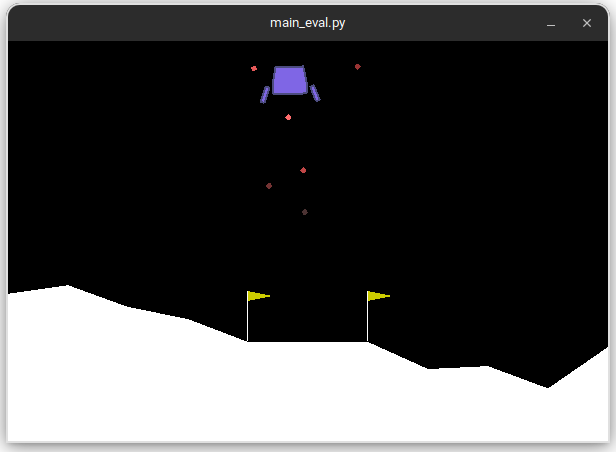
\includegraphics[width=\columnwidth]{./img/lunar-lander-env.png}}
    \caption{The Lunar Lander environment.}
    \label{fig:lunar-lander-env}
\end{figure}


%%%%%%%%%%%%%%%%%%%%%%%%%%%%%%%%%%%%%%%%%%%%%%%%%%%%%%%%%%%%%%%%%%%%%%%%%%%%%%%%%%%%%%%%%%%%%%%%%%%%%%%%%%%
\subsection{Acrobot}

The Acrobot environment\footnote{Acrobot: \url{https://www.gymlibrary.dev/environments/classic_control/acrobot}} shown in Figure \ref{fig:acrobot-env} is a 2-link pendulum with only the second joint actuated, offered by OpenAI Gym \cite{brockman2016openai}. The goal is to swing the end of the pendulum up to a given height. The environment is based on the work of Sutton and Barto \cite{sutton2018reinforcement}.

The state space of the environment is a 6-dimensional vector containing the sin and cos of the two joint angles and the joint angular velocities. The action space is a single discrete scalar with values ranging from 0 to 5, corresponding to the following actions: apply +1, 0, or -1 torque to the actuated joint.

The reward structure of the environment is designed to encourage the agent to reach the goal height. At each timestep, the agent receives a reward of -1 for each step that does not reach the goal. If the goal is reached, the agent receives a reward of 0. The episode ends when the agent reaches the goal height or if the episode exceeds the maximum number of timesteps.

\begin{figure}[htbp]
    \centerline{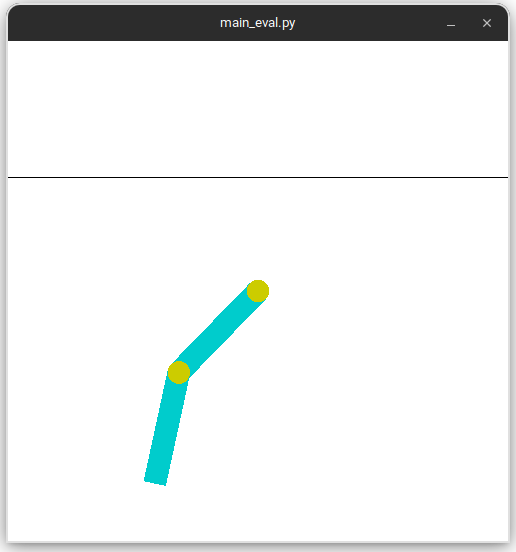
\includegraphics[width=\columnwidth]{./img/acrobot-env.png}}
    \caption{The Acrobot environment.}
    \label{fig:acrobot-env}
\end{figure}

%%%%%%%%%%%%%%%%%%%%%%%%%%%%%%%%%%%%%%%%%%%%%%%%%%%%%%%%%%%%%%%%%%%%%%%%%%%%%%%%%%%%%%%%%%%%%%%%%%%%%%%%%%%
\subsection{Bipedal Walker}
%. There are no coordinates in the state vector.


The Bipedal Walker environment\footnote{Bipedal Walker: \url{https://www.gymlibrary.dev/environments/box2d/bipedal_walker}} shown in Figure \ref{bipedal-walker-env} is a challenging control task offered by OpenAI Gym \cite{brockman2016openai}. The goal is to control a two-legged robot to walk as far as possible without falling. This environment has continuous action and state spaces, making it more challenging than the discrete action spaces of the Lunar Lander and Acrobot environments.

The state space of the environment is a 24-dimensional vector containing the position, velocity, and angle of the robot's body and legs. The action space is a continuous 4-dimensional vector, with each dimension representing the torque applied to one of the robot's joints.

The reward structure of the environment is designed to encourage the robot to move forward without falling. The robot receives a reward of +1 for each timestep it is able to remain upright and move forward. If the robot falls, it receives a large negative reward. The episode ends when the robot falls or reaches the maximum number of timesteps.

Overall, the BipedalWalker environment presents a more challenging control task for our reinforcement learning agents compared to the Lunar Lander and Acrobot environments. This allows us to evaluate the performance of our agents on a wider range of tasks and environments.

\begin{figure}[htbp]
    \centerline{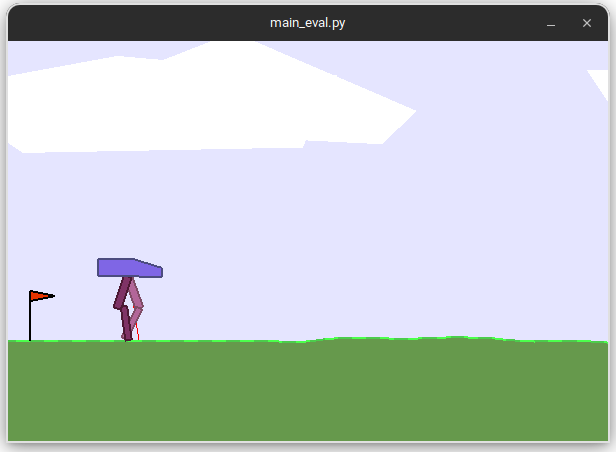
\includegraphics[width=\columnwidth]{./img/bipedal-walker-env.png}}
    \caption{The Bipedal Walker environment.}
    \label{bipedal-walker-env}
\end{figure}

%%%%%%%%%%%%%%%%%%%%%%%%%%%%%%%%%%%%%%%%%%%%%%%%%%%%%%%%%%%%%%%%%%%%%%%%%%%%%%%%%%%%%%%%%%%%%%%%%%%%%%%%%%%
%%%%%%%%%%%%%%%%%%%%%%%%%%%%%%%%%%%%%%%%%%%%%%%%%%%%%%%%%%%%%%%%%%%%%%%%%%%%%%%%%%%%%%%%%%%%%%%%%%%%%%%%%%%
\section{Methodology}

Our agents implement the Proximal Policy Optimization (PPO) algorithm to learn the optimal policy for each environment. PPO is a popular policy gradient method that uses a clipped surrogate objective function to improve the policy.

To train the PPO algorithm, we generate trajectory samples by keeping track of both the states and actions of the environment, as well as the outputs of the network for each sample in the trajectory. We then use these trajectory samples to train the network in batches, where each batch of data is used to run several training steps. The number of training steps of optimization that we run for each batch of data is defined as a configurable hyperparameter.

The network architecture used by our agents is composed of two main components: the actor and the critic. The actor part of the network generates the policy distribution for the state-action pairs, while the critic uses the Generative Pre-trained Transformer 2 (GPT2) model as an encoder to generate predictions for the state-action pairs and generate the value function.

To prevent the actor network from overfitting, we use a simpler feed-forward network that only takes in the last state of the trajectory as input. This allows the agent to continue exploring the environment and avoids overfitting, while the critic network uses the full sequence data to make more informed predictions about the actor's behavior over time and under specific conditions.

%%%%%%%%%%%%%%%%%%%%%%%%%%%%%%%%%%%%%%%%%%%%%%%%%%%%%%%%%%%%%%%%%%%%%%%%%%%%%%%%%%%%%%%%%%%%%%%%%%%%%%%%%%%
%%%%%%%%%%%%%%%%%%%%%%%%%%%%%%%%%%%%%%%%%%%%%%%%%%%%%%%%%%%%%%%%%%%%%%%%%%%%%%%%%%%%%%%%%%%%%%%%%%%%%%%%%%%
%Reinforcement Learning Methods(5%)
%Describe the reinforcement method/methods you are planning to use in this work. This
%should give the background for the methods. If you are comparing multiple ones, make
%sure to describe them all. Feel free to add diagrams and equations to clarify.

\subsection{Reinforcement Learning Methods}

In this project, we use the Proximal Policy Optimization (PPO) algorithm \cite{schulman2017proximal} to find the optimal policies for agents to follow in unknown environments. PPO is a state-of-the-art reinforcement learning algorithm that is both effective and efficient. It works by using a policy to determine the actions that an agent should take in a given state, and then using a value function to evaluate the potential outcomes of those actions. The algorithm then uses this information to adjust the policy in a way that maximizes the expected reward for the agent.

We use the PPO-clip variant of the algorithm, which uses a "clipping" mechanism to prevent the algorithm from making too large of a change to the policy in a single iteration. This helps to stabilize the learning process and prevent the algorithm from becoming too "jumpy" or erratic.

In addition to the PPO algorithm, we also use the transformer architecture \cite{attentionisallyouneed} as part of our network. The transformer is a type of neural network architecture that is commonly used in natural language processing tasks, such as machine translation and text summarization. It is able to process large amounts of data very efficiently, and uses self-attention mechanisms to "focus" on different parts of the input data at different times.

In the context of our PPO algorithm, the transformer is used to generate predictions for the state-action pairs. The transformer takes in the sequence of state-action pairs as input, and then uses self-attention to capture long-term dependencies in the data. The output of the transformer is then used by the critic head of the network to generate the value function, which is used to evaluate the potential outcomes of the actions taken by the agent.

Overall, our approach to reinforcement learning combines the powerful PPO algorithm with the efficient transformer architecture to learn the optimal policies for agents in unknown environments. This allows us to take advantage of the strengths of both methods.

%%%%%%%%%%%%%%%%%%%%%%%%%%%%%%%%%%%%%%%%%%%%%%%%%%%%%%%%%%%%%%%%%%%%%%%%%%%%%%%%%%%%%%%%%%%%%%%%%%%%%%%%%%%
%%%%%%%%%%%%%%%%%%%%%%%%%%%%%%%%%%%%%%%%%%%%%%%%%%%%%%%%%%%%%%%%%%%%%%%%%%%%%%%%%%%%%%%%%%%%%%%%%%%%%%%%%%%
%Code Design(5%)
%Describe the general structure of your code including functions, classes, and data struc-
%tures used. If you are using code written by someone else make sure to cite it and
%emphasize the parts that you have written yourself.

\section{Code Design}

%%%%%%%%%%%%%%%%%%%%%%%%%%%%%%%%%%%%%%%%%%%%%%%%%%%%%%%%%%%%%%%%%%%%%%%%%%%%%%%%%%%%%%%%%%%%%%%%%%%%%%%%%%%
\subsection{Utilized Libraries}


One of the main libraries we use in this work is PyTorch \cite{paszke2019pytorch}. PyTorch is a popular deep learning library that is well-documented and has a large community. We chose to use PyTorch because it is easy to use and has a wide range of powerful tools for building and training deep learning models.

In addition to PyTorch, we also use the PyTorch-Lightning library \cite{falcon2019pytorch}. PyTorch-Lightning is a high-level library that makes it easy to train and test deep learning models. It provides a module named Lightning-Bolts that contains many pre-built models and utilities, which we use to help maintain the structure of our models.

To implement the GPT2 model, we use the HuggingFace Transformers library \cite{wolf2019huggingface}. This library provides an intuitive interface for working with the GPT2 model, allowing us to easily incorporate it into our reinforcement learning algorithms.

We use the OpenAI Gym library \cite{brockman2016openai} to provide the environments for our models to train and test on. The Gym library offers a wide range of environments that are well-suited to reinforcement learning tasks.

Finally, we use Weights \& Biases (WandB) \cite{wandb} to log the results of our experiments. WandB allows us to track and visualize the performance of our models over time, helping us to understand how they are performing and identify areas for improvement.

% In summary, these libraries are essential tools that help us to effectively and efficiently implement and evaluate our reinforcement learning algorithms.

%%%%%%%%%%%%%%%%%%%%%%%%%%%%%%%%%%%%%%%%%%%%%%%%%%%%%%%%%%%%%%%%%%%%%%%%%%%%%%%%%%%%%%%%%%%%%%%%%%%%%%%%%%%
\subsection{File Structure}

The main directory of this project contains the \textit{main\_train.py} and \textit{main\_eval.py} files. These files are used to train and test the models, respectively.

The core code is contained within the \textit{rllib} directory. Within this directory, there are many files that are important to the project. The primary files that are used are \textit{Model.py}, \textit{GPT2PPO.py}, \textit{CommonGPT2.py}, \textit{CommonBase.py}, and \textit{GPT2.py}. These files will be discussed in more detail in the following sections.

The \textit{rllib/examples} directory contains A2C and PPO baseline implementations that were taken from the Lightning-Bolts library and copied into our project.

Finally, the \textit{archive} directory holds all the iterations of old code that we have tried and discarded. This directory provides a history of our development process and helps us to keep track of what we have tried and why we made certain decisions.


%%%%%%%%%%%%%%%%%%%%%%%%%%%%%%%%%%%%%%%%%%%%%%%%%%%%%%%%%%%%%%%%%%%%%%%%%%%%%%%%%%%%%%%%%%%%%%%%%%%%%%%%%%%
\subsection{Training and Testing Tools}
To train a model, we use the \textbf{main\_train.py} file. This file will train a model on a given environment and log the results.
To train a model, we use the following command:
\begin{center}
    \texttt{python3 main\_train.py \textbackslash \\}
    \texttt{-m ppo\_gpt \textbackslash \\}
    \texttt{-e LunarLander-v2}
\end{center}

For the \textbf{main\_train.py} file we have the following additional command line arguments:
\begin{itemize}
    \item \texttt{-e} or \texttt{--env} - The Open AI Gym environment [Default: LunarLander-v2]
    \item \texttt{-m} or \texttt{--model\_name} - The name of the model to train [Default: ppo\_ex (PPO)]
    \item \texttt{-ne} or \texttt{--num\_epochs} - The number of epochs to train for [Default: 150]
    \item \texttt{--al\_check\_interval} - The interval of epochs to run validation [Default: 5]
    \item \texttt{--wandb\_project} - The wandb project to log to [Default: rl\_project]
    \item \texttt{--wandb\_entity} - The wandb entity to log to [Default: ece517]
    \item \texttt{--seed} - The seed value for training [Default: 123]
\end{itemize}

The training command will train the model then save the trained model to the checkpoints directory with the following structure:
\begin{center}
    \texttt{checkpoints/\\<model\_name>/\\<env\_name>/\\<model\_hash>.pt}
\end{center}

To test a model (watch it interact in the environment), we use the \textbf{main\_eval.py}. This file will load a model from the checkpoints directory and
run it in the environment.
To test a model, we use the following command:
\begin{center}
    \texttt{python3 main\_eval.py -f <model\_checkpoint>}
\end{center}

For the \textbf{main\_eval.py} file, we have the following additional command line arguments:
\begin{itemize}
    \item \texttt{-f} or \texttt{--file\_path} - The path to the model checkpoint
    \item \texttt{-ne} or \texttt{--num\_episodes} - The number of episodes to run [Default: 5]
    \item \texttt{--running\_rew\_len} - The length of rewards to store at once [Default: 50]
    \item \texttt{--seed} - The seed value for testing [Default: 123]
\end{itemize}

Both the \textbf{main\_train.py} and \textbf{main\_eval.py} files utilize the \textbf{rllib/Model.py} file.
This file abstracts the training and evaluation process from the training and testing commands into a class named Model.
It simply loads in the correct model and trains or tests it.

%%%%%%%%%%%%%%%%%%%%%%%%%%%%%%%%%%%%%%%%%%%%%%%%%%%%%%%%%%%%%%%%%%%%%%%%%%%%%%%%%%%%%%%%%%%%%%%%%%%%%%%%%%%
\subsection{Models}


In this work, we use the \textit{Proximal Policy Optimization (PPO)} algorithm to learn the optimal policies for agents in unknown environments. The baseline PPO model we use to compare against our results is in the \textit{rllib/examples/PPOExample.py} file. It contains code from the Lighting-Bolts library with no modifications. We store this model locally to protect against any future API changes in the library. The file contains a class named PPO that inherits from the LightningModule class. Our implementation is built upon this class.

Our implementation is in the \textit{rllib/GPT2PPO.py} file. This file contains the \textit{GPT2PPO} class which implements the same interface as the reference PPO. In addition to the MLP, ActorContinuous, and ActorCategorical models used in the baseline PPO implementation from the Lighting-Bolts library, we use two additional models implemented in the \textit{rllib/CommonBase.py} and \textit{rllib/CommonGPT2.py} files.

The \textit{rllib/CommonBase.py} file implements the \textit{CommonBase} class. This class implements a simple Sequential model containing a Linear layer with a ReLU activation function followed by a Linear layer with no activation function. This class is used as the base of the ActorCategorical and ActorContinuous models. States are fed through this and immediately given to the actor.

The \textbf{rllib/CommonGPT2.py} file implements the CommonGPT2 class. This class implements a usage of the GPT2 model which is stored in the \textbf{rllib/GPT2.py} file. The GPT2 model is taken from the Decision Transformer implementation\cite{chen2021decision}. In that work, the authors took the HuggingFace GPT2 model and removed the logic that implment positional embeddings\cite{radford2019language,wolf2019huggingface}. Our CommonGPT2 shares large similarities with the Decision Transformer implementation\cite{chen2021decision}; however, we chose to only feed the states and actions to GPT2 rather than the states, actions, and rewards to go. As input, CommonGPT2 will take a history of timesteps, states, and actions as input of shape (batch\_size, sequence\_length,:). It will then return an embedding of the state and action. The embedding of the state is then fed to the critic and the critic predicts the value of the state.

GPT2PPO has some differences from the baseline PPO in how the internals are structured. Because we are using a transformer, we need to keep track of the history of the states, actions, timesteps, and attention masks used by the model. We do this by storing each of the respective histories in a buffer of a length equal to the context length of the GPT2 model. When the buffer is full, the oldest entry is removed, and the new entry is added to the end of the buffer. The buffer is then fed to the GPT2 model, and the most current state is fed through the CommonBase and then the actor. The GPT2 model will then return an embedding of the state and action. The embedding of the state is given to the critic. All inputs are saved in a history array which is later used for training.

There are two main functions for data generation and training. The \textbf{generate\_trajectory\_samples} function is used to generate data for training. It runs a configured number of timesteps then yields the model inputs, attention masks, actions, log probabilities, Q values, and Advantages for all timesteps. The \textbf{training\_step} function takes a batch of data and calculates and returns the loss for the actor or critic. This loss is used by the Pytorch-Lightning framework to update the actor or critic.

% TODO probably more detail can be added.

%%%%%%%%%%%%%%%%%%%%%%%%%%%%%%%%%%%%%%%%%%%%%%%%%%%%%%%%%%%%%%%%%%%%%%%%%%%%%%%%%%%%%%%%%%%%%%%%%%%%%%%%%%%
%%%%%%%%%%%%%%%%%%%%%%%%%%%%%%%%%%%%%%%%%%%%%%%%%%%%%%%%%%%%%%%%%%%%%%%%%%%%%%%%%%%%%%%%%%%%%%%%%%%%%%%%%%%
%Results Analysis(40%)
%Present the results which answer your hypothesis questions. These should include dif-
%ferent graphs which clarify the answer and examine different aspects of your solution.
%Make sure to carefully describe how your experiments were conducted (how many runs,
%how it was initialized, etc. This section is the most important, and will be evaluated
%both on presentation and correctness.


\section{Results}
\label{sec:results}

In this work, we compare the results of our GPT2PPO model against the baseline PPO model. We compare the results of both models on the Lunar Lander, Acrobot, and environments. To keep all of our results consistent, when comparing models, we ran each model with the same hyperparameters for the same number of epochs. The hyperparameters for both models are listed in Table \ref{tab:hyperparameters}. We ran each model 3 times and averaged the results.

\begin{table}[htbp]
    \caption{Model Hyperparameters}
    \begin{center}
        \begin{tabular}{|c|c|}
            \hline
            \multicolumn{2}{|c|}{\textbf{Hyperparameters}}     \\
            \hline
            \textbf{Param}           & \textbf{\textit{Value}} \\
            \hline
            Environment Seed         & 123                     \\
            Epochs                   & 150                     \\
            Gamma                    & 0.99                    \\
            Lambda                   & 0.95                    \\
            Batch Size               & 128                     \\
            Actor Learning Rate      & 3e-4                    \\
            Critic Learning Rate     & 1e-3                    \\
            Max Episode Length       & 500                     \\
            Steps Per Epoch          & 2048                    \\
            Training Steps Per Epoch & 5                       \\
            Clip Ratio               & 0.2                     \\
            Hidden Size              & 64                      \\
            Context Length*          & 64                      \\
            Number of Layers*        & 2                       \\
            Number of Heads*         & 8                       \\
            Dropout*                 & 0.5                     \\
            Number of Positions*     & 1024                    \\
            \hline
            \multicolumn{2}{l}{*Only used for GPT2PPO.}
        \end{tabular}
        \label{tab:hyperparameters}
    \end{center}
\end{table}

%%%%%%%%%%%%%%%%%%%%%%%%%%%%%%%%%%%%%%%%%%%%%%%%%%%%%%%%%%%%%%%%%%%%%%%%%%%%%%%%%%%%%%%%%%%%%%%%%%%%%%%%%%%
\subsection{Lunar Lander}

Lunar Lander is a simple environment that we assume will be easy for both models to learn. We do not believe recurrence or attention will offer any superior advantage to base PPO in this environment. As described above, we trained both PPO and GPT2PPO for 150 epochs three times and averaged the results. Through our experiments, we found the models to be comparable in performance.

Figure \ref{lunar-lander-loss_critic-model} shows the critic loss for both models. It can be seen that the GPT2PPO model critic learns slower than the Baseline PPO model. This is likely due to the fact that the GPT2PPO model has far more weights to train, and the input to the model is much larger. However, the GPT2PPO critic does learn and eventually converges to a similar critic loss as the baseline PPO model.

Figure \ref{lunar-lander-loss_actor-model} shows the actor loss for both models. It can be seen that the loss for both models is very similar. This is likely because the actor in both models is very similar. The only difference is that the actor has two additional layers.

Figure \ref{lunar-lander-avg_ep_reward-model} shows the average episode reward for both models. On average, the GPT2PPO model gains increases in average episode rewards at a similar pace as the Baseline PPO. However, the GPT2PPO model does not reach the same average reward as the Baseline PPO model; instead, it converges upon a slightly lower episode reward.

Figure \ref{lunar-lander-avg_ep_len-model} shows the average episode length for both models. On average, the GPT2PPO model gains increases in average episode length slower than the Baseline PPO. Additionally, the GPT2PPO model does not reach the same average episode length as the Baseline PPO model. The GPT2PPO model seems to learn up to a certain point but fails to converge upon an optimal policy. This could be because we needed to train the model for more epochs
Overall, the GPT2PPO model performs similarly to the baseline PPO model. However, the GPT2PPO model converges to slightly worse values as compared to the Baseline PPO model.

%% PPO vs GPT2PPO - Comparison
\begin{figure}[htbp]
    \centerline{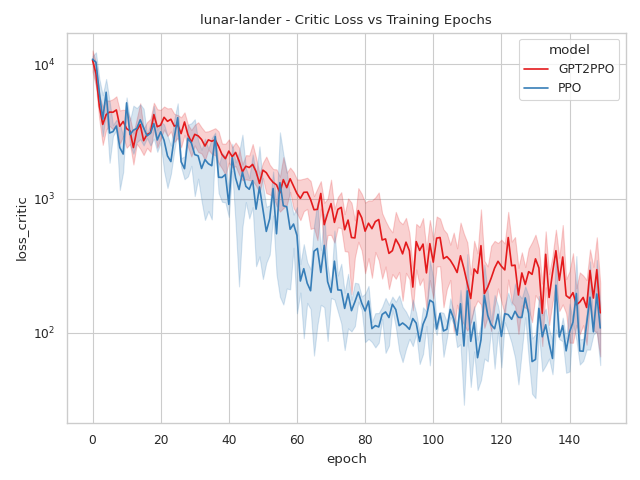
\includegraphics[width=\columnwidth]{./img/lunar-lander-loss_critic-model.png}}
    \caption{Lunar Lander - PPO vs GPT2PPO - Critic Loss}
    \label{lunar-lander-loss_critic-model}
\end{figure}
\begin{figure}[htbp]
    \centerline{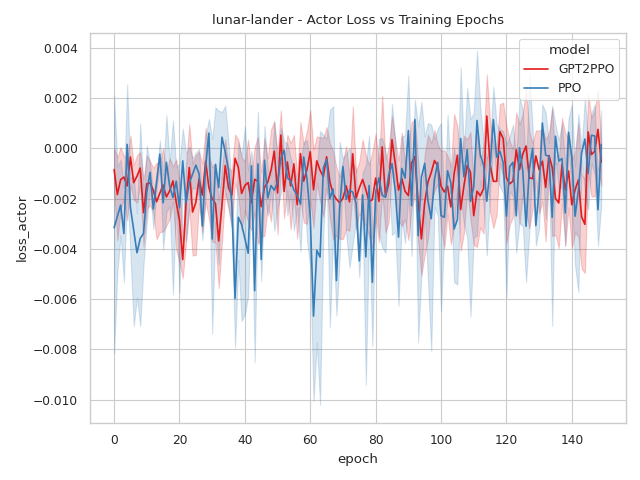
\includegraphics[width=\columnwidth]{./img/lunar-lander-loss_actor-model.png}}
    \caption{Lunar Lander - PPO vs GPT2PPO - Actor Loss}
    \label{lunar-lander-loss_actor-model}
\end{figure}
\begin{figure}[htbp]
    \centerline{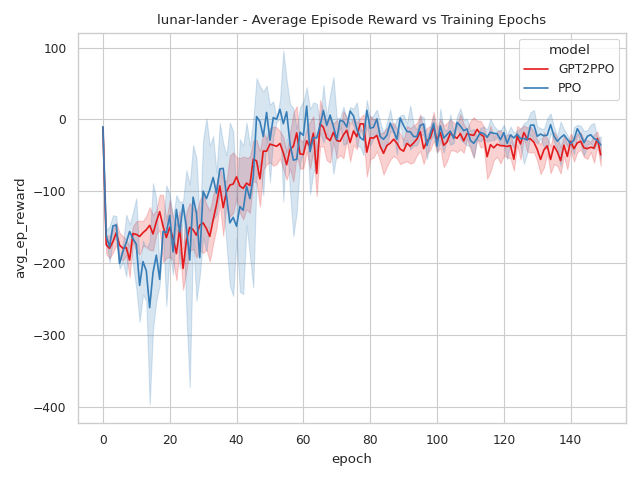
\includegraphics[width=\columnwidth]{./img/lunar-lander-avg_ep_reward-model.png}}
    \caption{Lunar Lander - PPO vs GPT2PPO - Average Episode Reward}
    \label{lunar-lander-avg_ep_reward-model}
\end{figure}
\begin{figure}[htbp]
    \centerline{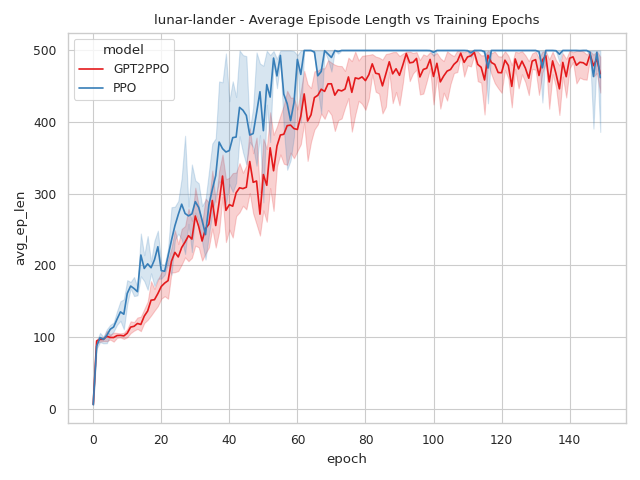
\includegraphics[width=\columnwidth]{./img/lunar-lander-avg_ep_len-model.png}}
    \caption{Lunar Lander - PPO vs GPT2PPO - Average Episode Length}
    \label{lunar-lander-avg_ep_len-model}
\end{figure}


We also experimented with different context lengths for the GPT2PPO model for the Lunar Lander environment. We kept the same hyperparameters shown in Table \ref{tab:hyperparameters}, but altered the context length to be 25, 50, and 75.
Figures \ref{lunar-lander-loss_critic-ctx_len}, \ref{lunar-lander-loss_actor-ctx_len}, \ref{lunar-lander-avg_ep_reward-ctx_len}, and \ref{lunar-lander-avg_ep_len-ctx_len} show these results. We can see that all context lengths perform similarly. This is likely because of the structure of the environment.

%% GPT2PPO - Different Context Lengths
% Context lengths of [25,50,75]
\begin{figure}[htbp]
    \centerline{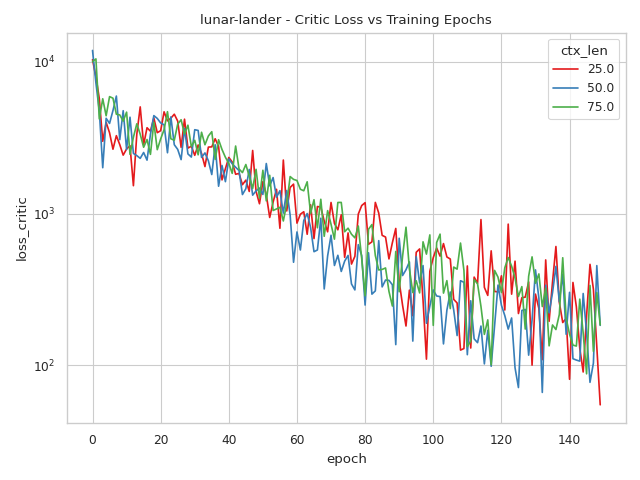
\includegraphics[width=\columnwidth]{./img/lunar-lander-loss_critic-ctx_len.png}}
    \caption{Lunar Lander - GPT2PPO Context Length - Critic Loss}
    \label{lunar-lander-loss_critic-ctx_len}
\end{figure}

\begin{figure}[htbp]
    \centerline{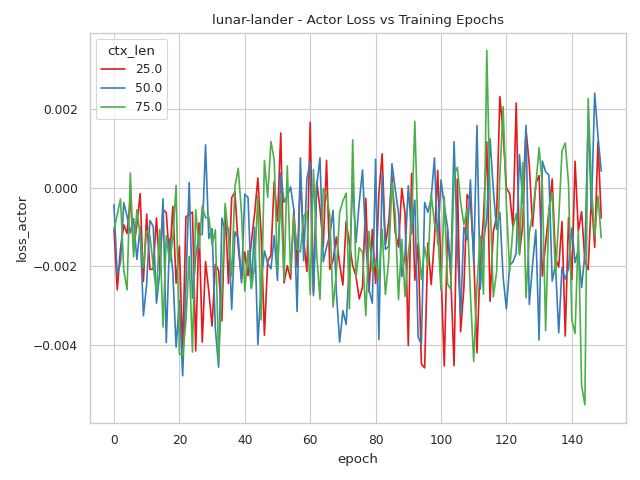
\includegraphics[width=\columnwidth]{./img/lunar-lander-loss_actor-ctx_len.png}}
    \caption{Lunar Lander - GPT2PPO Context Length - Actor Loss}
    \label{lunar-lander-loss_actor-ctx_len}
\end{figure}

\begin{figure}[htbp]
    \centerline{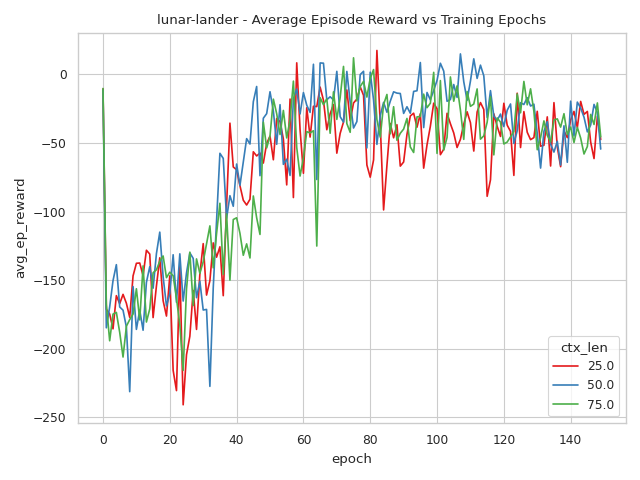
\includegraphics[width=\columnwidth]{./img/lunar-lander-avg_ep_reward-ctx_len.png}}
    \caption{Lunar Lander - GPT2PPO Context Length - Average Episode Reward}
    \label{lunar-lander-avg_ep_reward-ctx_len}
\end{figure}

\begin{figure}[htbp]
    \centerline{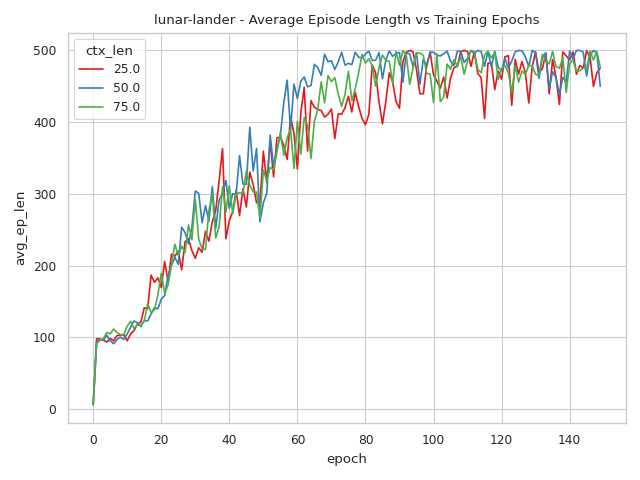
\includegraphics[width=\columnwidth]{./img/lunar-lander-avg_ep_len-ctx_len.png}}
    \caption{Lunar Lander - GPT2PPO Context Length - Average Episode Length}
    \label{lunar-lander-avg_ep_len-ctx_len}
\end{figure}

%%%%%%%%%%%%%%%%%%%%%%%%%%%%%%%%%%%%%%%%%%%%%%%%%%%%%%%%%%%%%%%%%%%%%%%%%%%%%%%%%%%%%%%%%%%%%%%%%%%%%%%%%%%
\subsection{Acrobot}
The Acrobot environment is slightly more complex than the Lunar Lander environment. We stipulate that some sense of recurrence or attention would be beneficial as the agent should likely take into account its previous states and actions when making a decision to conserve its momentum. Through our experiments, we find that the GPT2PPO model tends to learn faster than the Baseline PPO model but tends to converge to poorer values. Additionally, we found that our model is hugely dependent on starting conditions of the GPT2 model.

Figure \ref{acrobot-loss_critic-model} shows the critic loss for both models. We can see that the GPT2PPO model learns faster on average than the Baseline PPO model, but after 90 epochs, it will diverge to a worse value. Figure \ref{acrobot-loss_actor-model} shows the actor loss for both models. The average results are similar between each model. Our model seems to have a higher variance as compared to the Baseline PPO model.

Figure \ref{acrobot-avg_ep_reward-model} shows the average episode reward for both models. The shaded regions show the minimum and maximum values for each model across the three runs. Here we can see that the results for our model vary. Our model's minimum average episode reward stays equal to the maximum episode length of 500. It does not seem to improve until the 90th epoch, where it quickly improves toward the results of other runs. On the other side of the spectrum, the maximum average episode reward learns much quicker than the Baseline PPO model. Moreover, our model, on average, will learn at a similar pace to the Baseline PPO model but will converge to a worse value.

%% PPO vs GPT2PPO - Comparison
\begin{figure}[htbp]
    \centerline{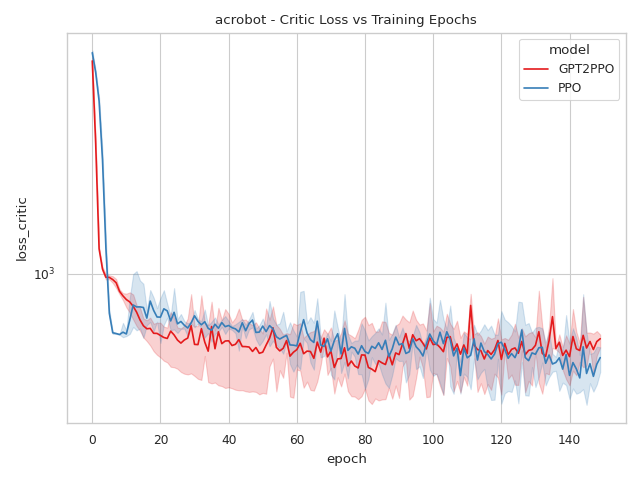
\includegraphics[width=\columnwidth]{./img/acrobot-loss_critic-model.png}}
    \caption{Acrobot - PPO vs GPT2PPO - Critic Loss}
    \label{acrobot-loss_critic-model}
\end{figure}

\begin{figure}[htbp]
    \centerline{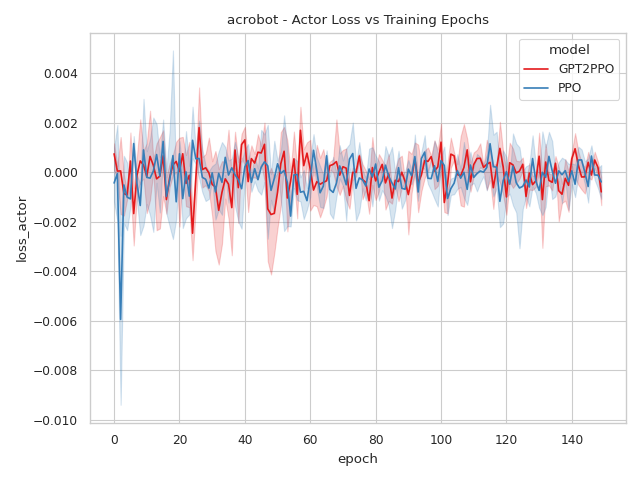
\includegraphics[width=\columnwidth]{./img/acrobot-loss_actor-model.png}}
    \caption{Acrobot - PPO vs GPT2PPO - Actor Loss}
    \label{acrobot-loss_actor-model}
\end{figure}

\begin{figure}[htbp]
    \centerline{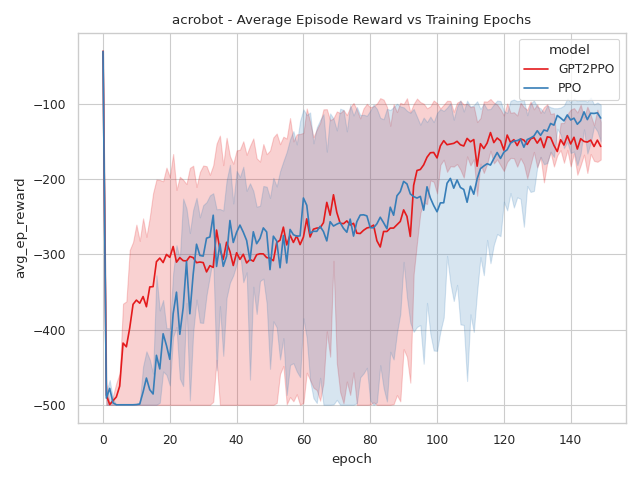
\includegraphics[width=\columnwidth]{./img/acrobot-avg_ep_reward-model.png}}
    \caption{Acrobot - PPO vs GPT2PPO - Average Episode Reward}
    \label{acrobot-avg_ep_reward-model}
\end{figure}

% \begin{figure}[htbp]
%     \centerline{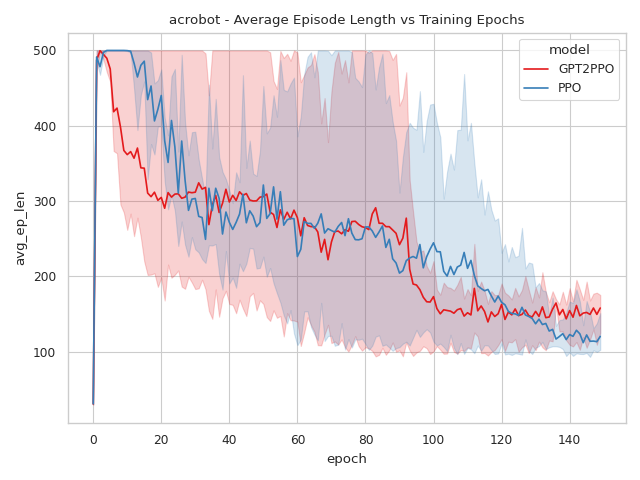
\includegraphics[width=\columnwidth]{./img/acrobot-avg_ep_len-model.png}}
%     \caption{Acrobot - PPO vs GPT2PPO - Average Episode Length}
%     \label{acrobot-avg_ep_len-model}
% \end{figure}

%%%%%%%%%%%%%%%%%%%%%%%%%%%%%%%%%%%%%%%%%%%%%%%%%%%%%%%%%%%%%%%%%%%%%%%%%%%%%%%%%%%%%%%%%%%%%%%%%%%%%%%%%%%
\subsection{Bipedal Walker}
The Bipedal Walker represents the most complex environment we have trained our model on. This is because the state space is large, and the action space is continuous. We hypothesize that the configuration of our model used to compare against the Baseline PPO is insufficient to learn the environment. To learn better, we would need to increase the size of the GPT2 model and the number of epochs.

Figure \ref{bipedal-walker-loss_critic-model} shows the critic loss for both models. We can see that the converged GPT2PPO critic loss is higher than the Baseline PPOs by a factor of 10. This is consistent with Figure \ref{bipedal-walker-loss_actor-model}, where the GPT2PPO actor loss is a factor of 1000 higher than the converged Baseline PPO actor loss. Figure \ref{bipedal-walker-avg_ep_reward-model} shows the average episode reward for both models. Similar to the Acrobot environment, the results of our model significantly vary. Our model quickly switches between good and bad policies, whereas the Baseline PPO model converges much more smoothly.
Overall, the Baseline PPO model significantly outperforms our model in this environment.

\begin{figure}[htbp]
    \centerline{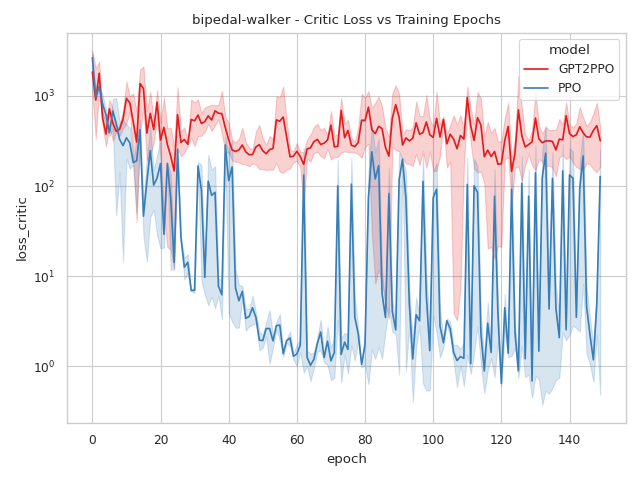
\includegraphics[width=\columnwidth]{./img/bipedal-walker-loss_critic-model.png}}
    \caption{Bipedal Walker - PPO vs GPT2PPO - Critic Loss}
    \label{bipedal-walker-loss_critic-model}
\end{figure}

\begin{figure}[htbp]
    \centerline{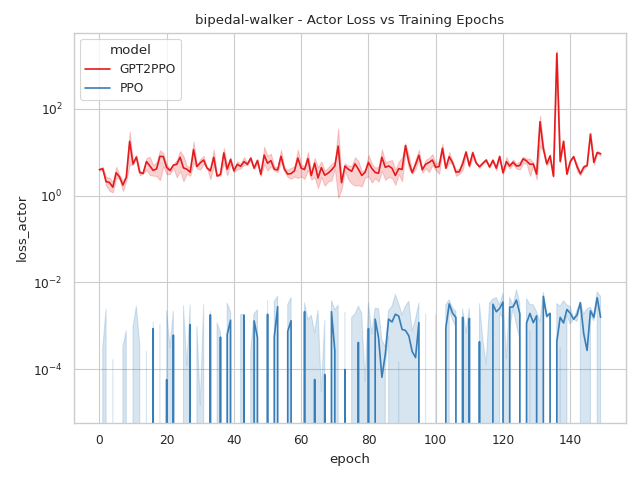
\includegraphics[width=\columnwidth]{./img/bipedal-walker-loss_actor-model.png}}
    \caption{Bipedal Walker - PPO vs GPT2PPO - Actor Loss}
    \label{bipedal-walker-loss_actor-model}
\end{figure}

\begin{figure}[htbp]
    \centerline{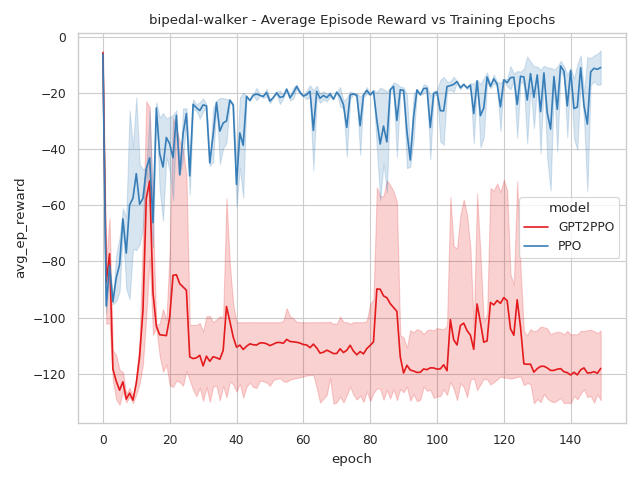
\includegraphics[width=\columnwidth]{./img/bipedal-walker-avg_ep_reward-model.png}}
    \caption{Bipedal Walker - PPO vs GPT2PPO - Average Episode Reward}
    \label{bipedal-walker-avg_ep_reward-model}
\end{figure}

% \begin{figure}[htbp]
%     \centerline{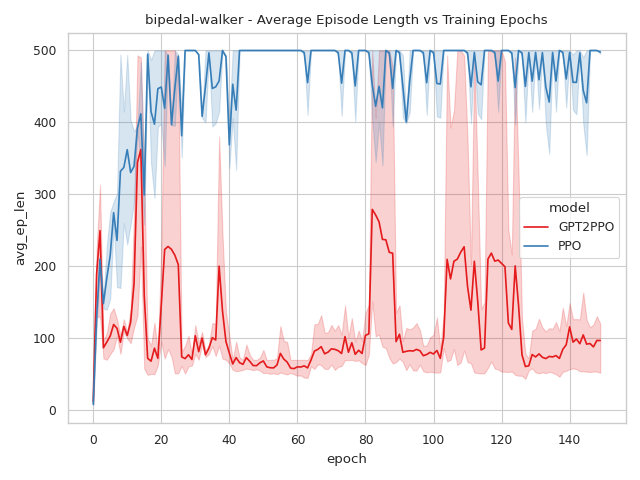
\includegraphics[width=\columnwidth]{./img/bipedal-walker-avg_ep_len-model.png}}
%     \caption{Bipedal Walker - PPO vs GPT2PPO - Average Episode Length}
%     \label{bipedal-walker-avg_ep_len-model}
% \end{figure}

%%%%%%%%%%%%%%%%%%%%%%%%%%%%%%%%%%%%%%%%%%%%%%%%%%%%%%%%%%%%%%%%%%%%%%%%%%%%%%%%%%%%%%%%%%%%%%%%%%%%%%%%%%%
%%%%%%%%%%%%%%%%%%%%%%%%%%%%%%%%%%%%%%%%%%%%%%%%%%%%%%%%%%%%%%%%%%%%%%%%%%%%%%%%%%%%%%%%%%%%%%%%%%%%%%%%%%%
%Conclusion(5%)
%What have you achieved in this project? What have you learned?

\section{Conclusion}
\label{sec:conclusion}


In this work, we propose an addition to the Proximal Policy Optimization (PPO) algorithm used in reinforcement learning, named GPT2PPO. This addition includes adding two layers to the actor network and an autoregressive model (GPT2) to the base of the critic network. We show that in simple environments, our model performs similarly to the basic PPO implementation but ultimately converges to a slightly poorer outcome. We also show that our model can learn in more complex environments, but additional model finetuning and training are needed to be effective in those environments.

When using a shared network layer for both the actor and critic, we find that the critic loss converges faster than the Baseline PPO, but the actor loss diverges after a small number of epochs. If given more time, we would like to validate the correctness of the model's inputs and outputs, finetune our model, and experiment on more environments to determine the viability of our approach.

Overall, we have learned about the inner workings of PPO and that applying attention in the form of transformers can be effective when done correctly. However, more work is needed to optimize our network architecture for complex environments.


%%%%%%%%%%%%%%%%%%%%%%%%%%%%%%%%%%%%%%%%%%%%%%%%%%%%%%%%%%%%%%%%%%%%%%%%%%%%%%%
%%%%%%%%%%%%%%%%%%%%%%%%%%%%%%%%%%%%%%%%%%%%%%%%%%%%%%%%%%%%%%%%%%%%%%%%%%%%%%%
% References
\bibliographystyle{IEEEtran}
\bibliography{main}

%%%%%%%%%%%%%%%%%%%%%%%%%%%%%%%%%%%%%%%%%%%%%%%%%%%%%%%%%%%%%%%%%%%%%%%%%%%%%%%
%%%%%%%%%%%%%%%%%%%%%%%%%%%%%%%%%%%%%%%%%%%%%%%%%%%%%%%%%%%%%%%%%%%%%%%%%%%%%%%
% An appendix describing which part of the project each team member was in charge of.
\appendix
\subsection{Team Member Contributions}
%%%%%%%%%%%%%%%%%%%%%%%%%%%%%%%%%%%%%%%%%%%%%%%%%%%%%%%%%%%%%%%%%%%%%%%%%%%%%%%

\textbf{Andrei Cozma}. text here.

%%%%%%%%%%%%%%%%%%%%%%%%%%%%%%%%%%%%%%%%%%%%%%%%%%%%%%%%%%%%%%%%%%%%%%%%%%%%%%%

\textbf{Hunter Price} contributed a working modification of the Decision Transformer that used only the time steps, states, and actions. He utilized Andrei's modification of PPO that stored a buffer of the past timesteps, states, and actions to feed to the CommonGPT2 model. He then modified this code to use consistent matrix shapes. He also added the ability for GPT2PPO to support continuous action spaces. He worked with Andrei to set up the training and testing framework in PyTorch. He found the baseline A2C and PPO implementation in the Lighting-Bolt library. He worked with Andrei to run many experiments used and shown in the report. He wrote code to visualize the results outside of WandB and save them locally. Worked with Andrei to write the report. Additionally, He ran many experiments with different versions of PPO, such as using VGG16 as a base for both the actor and critic when working with environments that gave image data as the state and a model that used a shared encoder with both the actor and critic networks.

%%%%%%%%%%%%%%%%%%%%%%%%%%%%%%%%%%%%%%%%%%%%%%%%%%%%%%%%%%%%%%%%%%%%%%%%%%%%%%%
%%%%%%%%%%%%%%%%%%%%%%%%%%%%%%%%%%%%%%%%%%%%%%%%%%%%%%%%%%%%%%%%%%%%%%%%%%%%%%%

\end{document}
